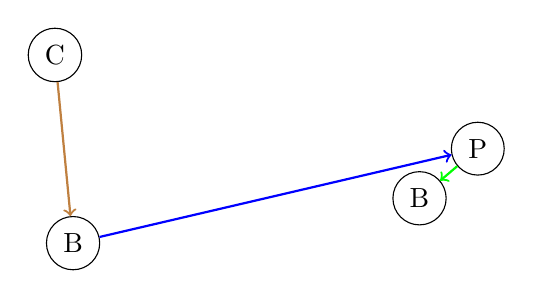
\begin{tikzpicture}
\node[circle, draw=black] (a) at (-0.61, -1.90) {C};
\node[circle, draw=black] (b) at (-0.38, -4.29) {B};
\node[circle, draw=black] (c) at (4.76, -3.09) {P};
\node[circle, draw=black] (d) at (4.02, -3.72) {B};
\draw[->, thick, brown] (a) -- (b);
\draw[->, thick, blue] (b) -- (c);
\draw[->, thick, green] (c) -- (d);
\end{tikzpicture}